\documentclass[a4paper, 11pt]{article}
\usepackage[utf8]{inputenc}
\usepackage[ngerman]{babel}
\usepackage{graphicx}
\usepackage{color}
\usepackage{xcolor}
\usepackage{wrapfig}
\usepackage{listings}
\usepackage{url, hyphenat}
\usepackage{hyperref}




\usepackage{color}
\usepackage{listings}
\usepackage{courier}

\parindent0mm
%\usepackage[margin=3cm]{geometry}

\clubpenalty=10000
\widowpenalty=10000


%\definecolor{gray}{model}{color-spec}


\lstset{
	basicstyle=\footnotesize\ttfamily, % Standardschrift
%	numbers=left, % Ort der Zeilennummern
	numberstyle=\tiny, % Stil der Zeilennummern
	numbersep=5pt, % Abstand der Nummern zum Text
	tabsize=2, % Groesse von Tabs
	extendedchars=true, %
	breaklines=true, % Zeilen werden Umgebrochen
	keywordstyle=\color{orange}\bfseries,
	frame=b,
	% keywordstyle=[1]\textbf, % Stil der Keywords
	% keywordstyle=[2]\textbf, %
	% keywordstyle=[3]\textbf, %
	% keywordstyle=[4]\textbf, \sqrt{\sqrt{}} %
	stringstyle=\color{blue!60!green}\ttfamily, % Farbe der String
	showspaces=false, % Leerzeichen anzeigen ?
	showtabs=false, % Tabs anzeigen ?
	xleftmargin=17pt,
	framexleftmargin=17pt,
	framexrightmargin=5pt,
	framexbottommargin=4pt,
	commentstyle=\color{gray},%\color{8},
	%backgroundcolor=\color{grey},
	showstringspaces=false, % Leerzeichen in Strings anzeigen ?
	morekeywords={TailCall}
}



\begin{document}
	
  \begin{titlepage}
  	\centering
  	
\includegraphics[width=\linewidth]{Hska_logo}
  	
  	\vspace{3em}
  	{\scshape \Large Modellbasierte Softwareentwicklung}
  	
  	\vspace{1.5em}
  	{\huge Kompilierung funktionaler Sprachen für die Java Virtual Machine}
  	
  	\vspace{3em}
  	{\large Tim Essig}
  	
  	{\large 49683}

 	\vspace{3em}
 	%\today
 	22. Januar 2018
  \end{titlepage}

  
  \section{Stack-basierte Virtuelle Maschienen}
	
	Stack-Maschinen nutzen für die Ausführung eine Stack um ihre Zwischenergebnisse zu speichern. Register-Maschinen hingegen nutzen Register um diese Zwischenergebnisse zu speichern. Bekannte Beispiele hierfür sind die x86 CPUs oder AVR MCUs. 
	Da Stack-Maschinen ihre Werte direkt vom Stack nehmen, kommen dieses mit sehr geringen Befehlsgrößen aus, da keine Adressen für Quell- oder Zielregister angegeben werden müssen. Meist lässt sich ein einfacher ADD Befehl mit einem Byte darstellen
	
	\begin{lstlisting}
	iadd
	\end{lstlisting}
	
	wohingegen ein einfacher ADD Befehl im x86 Befehlssatz bereits 3 Byte benötigt. 
	
	\begin{lstlisting}
	add Zieloperand, Quelloperand
	\end{lstlisting}
	
	Das kommt daher, dass die Operation ihre Parameter(in diesem Fall zwei, es können jedoch auch mehr sein) direkt vom Stack nimmt, genau so sind auch Operanden vorstellbar, welche mehr als einen Rückgabewert auf den Stack legen.
	Konstanten werden meist mit einem separaten load Befehl auf den Stack gelegt. Auch das laden von Werten aus dem Speicher erfolgt meist über eigene Befehle, die ihr Ergebnis direkt auf den Stack legen.
	
	Diese Funktionsweise gleicht auch der UPN(umgekehrt Polnische Notation), welche ebenfalls mit einem Stack arbeitet und zunächst die Werte übergibt und anschließend die Operation, so ergibt die UPN \textit{1 2 +} das Ergebnis 1 + 2 = 3. Diese Funktionsweise funktioniert vor allem für Highlevel Sprachen sehr gut, da die meisten Operationen einfach in die UPN gebracht werden können. 

	Aus Gründen der Geschwindigkeit werden die beiden obersten Felder des Stacks oft als Register ausgelegt, welche direkt mit der ALU verbunden sind, so können Berechnungen schneller durchgeführt werden.
	
	\subsection{Vorteile der Stack-Maschinen}
	
	Stack-Maschinen haben Operanden, die meistens nur ein Byte benötigen, dadurch, dass das Laden und Schreiben in den Speicher meist separate Befehle sind, erhöht sich jedoch die Anzahl der Befehle wieder. In Summe ist der Bytecode jedoch trotzdem kleiner. Dies kommt gerade Geräten zu gute, die wenig internen Speicher haben, wie z.B. Embedded oder mobile Endgeräte. Auch wenn der Bytecode über schlechte Internetverbindungen übertragen werden soll, zahlt sich die geringere Codegröße aus. So basiert zum Beispiel WebAssembly auf einer Stack-Maschine.\footnote{WebAssembly; http://webassembly.org/} Die meisten Implementierungen besitzen zudem einen load/store Befehl der auf eine relative Adresse im Stack verweist und so den effektiven Zugriff auf lokale Variablen ermöglicht, ohne diese an eine Speicheradresse zu speichern. 
	
	
	Zudem sind Compiler für Stack-Maschinen vergleichsweise einfach zu schreiben. Betrachten wir den Ausdruck \textit{e1 + e2}. Um diesen zu kompilieren wird im wesentlichen eine Schablone verwendet, die wie folgt aussieht: 
	\lstset{language=JVMIS}
	\begin{lstlisting}
[Code zur Berechnung von e1]
[Code zur Berechnung von e2]
iadd //nimmt die zwei obersten Werte des Stacks
	\end{lstlisting}
	
	Sei nun \textit{e1=2} und \textit{e2=3} so wird daraus:
	\begin{lstlisting}
iconst_2
iconst_3
iadd //nimmt die zwei obersten Werte des Stacks
\end{lstlisting}

	Nun soll die Berechnung etwas komplexer werden und wir ersetzen \textit{e1=2} durch \textit{e1=2*4}.
	Die Berechnung von \textit{e1=2*4} seht wie folgt aus:
	\begin{lstlisting}
iconst_2
iconst_4
imul //nimmt die zwei obersten Werte des Stacks
	\end{lstlisting}
	
	Setzen wir dies nun an stelle von \textit{e1} in unsere Schablone ein, so ergibt sich folgender Bytecode:
	\begin{lstlisting}
iconst_2
iconst_4
imul //nimmt die zwei obersten Werte des Stacks
iconst_3
iadd //nimmt die zwei obersten Werte des Stacks
\end{lstlisting}
	
	Ein weiterer Vorteil von Stack-Maschinen ist der, dass sie leichter in Software realisierbar sind, als Register-Maschinen. Dies wird wohl auch einer der Gründe, wieso die JVM darauf basiert.
	
	
	%//TODO Performance? \url{https://en.wikipedia.org/wiki/Stack_machine#Performance_disadvantages_of_stack_machines}
	
  \section{JVM Architektur}
  In der Abbildung~\ref{fig:jvmarch} ist die Architektur der JVM abgebildet.\footnote{Quelle: \url{http://www.fh-wedel.de/~si/seminare/ws07/Ausarbeitung/05.jvm/jvm2.htm}} Darauf soll jedoch nur kurz eingegangen werden. Wie bekannt sein dürfte interpretiert die JVM Bytecode und ist als Stack-Maschine aufgebaut. Ein Compiler der gegen die JVM compilieren möchte, muss .class-Dateien erstellen, welche den Bytecode der einzelnen Klassen beinhaltet. Da die JVM Ursprünglich nur für die Ausführung von Java ausgelegt war, spiegelt sich dies natürlich auch im Instruction-Set wieder und so unterstützt die JVM wenig bis gar keine Befehle für z.B. dynamisch typisierte Sprachen oder funktionale Sprachen(Beispiel Pattern-Matching). Eine Ausnahme ist hier sicherlich \textit{invokedynamic} welches mit Java 7 Einzug in die JVM hielt\footnote{\url{https://www.javaworld.com/article/2860079/learn-java/invokedynamic-101.html}}, dieser Befehl dient dazu, die Performance von dynamischen Sprachen wie z.B. Groovy zu verbessern, da hierdurch weit weniger Boilerplait Code generiert werden muss und auch der JIT wesentlich effizienter arbeiten kann. 
  
  
  
  \begin{figure}[ht]
  	\centering
  	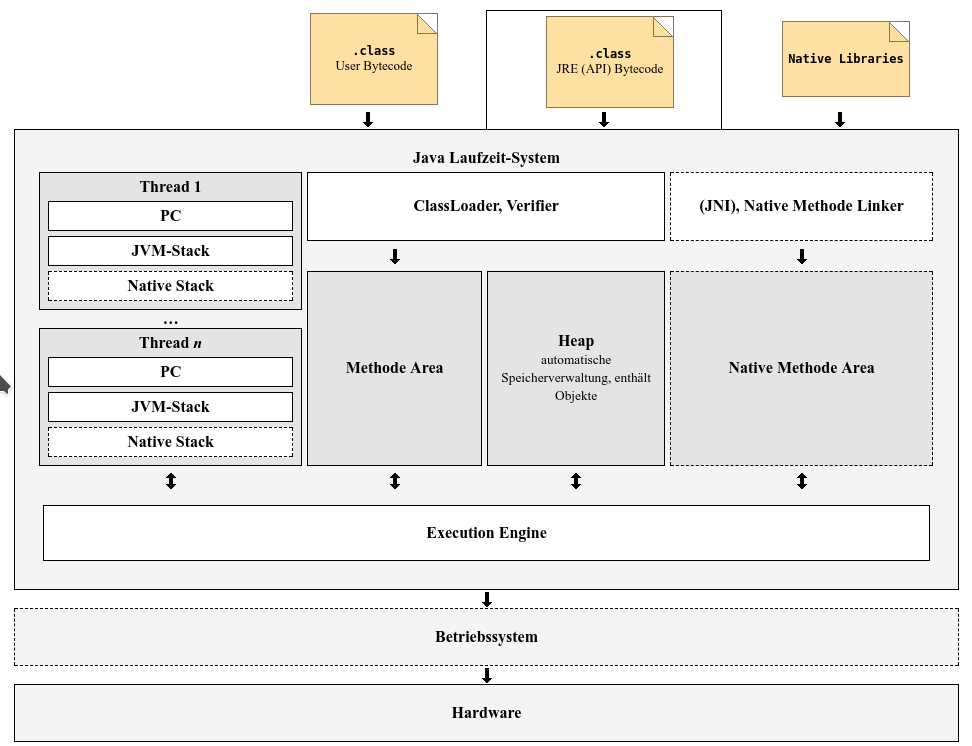
\includegraphics[width=1\linewidth]{JVM_Arch}
  	\caption{Architektur der JVMfoo}
  	\label{fig:jvmarch}
  \end{figure}

  
  	

  \subsection{Bytecode}
  Alle Sprachen die auf der JVM laufen wollen müssen in Bytecode übersetzt werden. Um im weiteren Kapitel zu verstehen, was für Code erzeugt wird, soll zunächst eine kleine Einführung in den Bytecode der JVM gegeben werden.
  
	\subsection{Decompilieren mit javap}
	Um das Resultat eines Compilers betrachten zu können, benötigen wir eine  Möglichkeit den Bytecode anzeige zu lassen. Hierzu bringt das JDK ein eigenes Tool mit \textit{javap}. Hiermit kann man sich die Struktur der *.class Dateien genauer anschauen. 
	Schauen wir uns eine Klasse an, die im späteren Kapitel noch einmal auftauchen wird.
    \lstset{language=Java}
	\begin{lstlisting}
public class TailCall {

  public static void main(String[] args) {
    System.out.println("Factor 3: " + factorial(3) );
  }

  static int factorial(int n) {
    if ( n == 0 )
      return 1;
    else
      return fact( n - 1, 1 );
  }

  static int fact(int i, int acc) {
    if ( i == 0 )
      return acc;
    else
      return fact( i - 1, acc * i);
  }
}
	\end{lstlisting}
	
	Nachdem wir die Klasse mit \textit{javac TailCall.java} compiliert haben, liefert uns der Befehl \textit{javap TailCall} folgendes Ergebnis:
\begin{lstlisting}
Compiled from TailCall.java
  public class TailCall {
    public TailCall();
    public static void main(java.lang.String[]);
    static int factorial(int);
    static int fact(int, int);
}
\end{lstlisting}
 Eine relativ einfache Darstellung des Inhalts des Classfiles. Wenn wir nun die Option \textit{-c} hinzufügen, so wird uns für die einzelnen Methoden nun auch der entsprechende Bytecode angezeigt:
 
 \lstset{language=JVMIS}
 \begin{lstlisting}
Compiled from "TailCall.java"
public class TailCall {
 public TailCall();
  Code:
    0: aload_0
    1: invokespecial #1 // Method java/lang/Object."<init>":()V
    4: return

 public static void main(java.lang.String[]);
  Code:
    0: getstatic     #2 // Field java/lang/System.out:Ljava/io/PrintStream;
    3: new           #3 // class java/lang/StringBuilder
    6: dup
    7: invokespecial #4 // Method java/lang/StringBuilder."<init>":()V
   10: ldc           #5 // String Factor 3:
   //...
   15: iconst_3
   16: invokestatic  #7 // Method factorial:(I)I
   //...
   25: invokevirtual #10 // Method java/io/PrintStream.println:(Ljava/lang/String;)V
   28: return

  static int factorial(int);
    Code:
      0: iload_0
      1: ifne          6
      4: iconst_1
      5: ireturn
      6: iload_0
      7: iconst_1
      8: isub
      9: iconst_1
     10: invokestatic  #11 // Method fact:(II)I
     13: ireturn

  static int fact(int, int);
    Code:
      0: iload_0
      1: ifne          6
      4: iload_1
      5: ireturn
      6: iload_0
      7: iconst_1
      8: isub
      9: iload_1
     10: iload_0
     11: imul
     12: invokestatic  #11 // Method fact:(II)I
     15: ireturn
}
 \end{lstlisting}
	Nun ist die Funktionsweise der Klasse schon sehr genau erkennbar, speziell, wie der Compiler diese in Bytecode umgesetzt hat.
	Auffällig sind die vielen Zahlen mit der führenden Raute, diese verweisen auf den \textit{Constant-Pool}.
	
	\subsection{Constant-Pool}
	Im \textit{Constant-Pool} werden alle benötigten Konstanten gespeichert. Wird \textit{javap} zusätzlich mit der Option \textit{-v} für Verbose aufgerufen, so wird dieser unter anderem auch angezeigt. Ein Ausschnitt der Ausgabe sieht wie folgt aus:
 \lstset{language=JVMIS}
\begin{lstlisting}
public class TailCall
minor version: 0
major version: 52
flags: (0x0021) ACC_PUBLIC, ACC_SUPER
this_class: #12                         // TailCall
super_class: #13                        // java/lang/Object
interfaces: 0, fields: 0, methods: 4, attributes: 1
Constant pool:
#1 = Methodref          #13.#27  // java/lang/Object...
#2 = Fieldref           #28.#29  // java/lang/System.out:Ljava/io/PrintStream;
#3 = Class              #30      // java/lang/StringBuilder
#4 = Methodref          #3.#27   // java/lang/StringBuilder...
#5 = String             #31      // Factor 3:
//...
#30 = Utf8               java/lang/StringBuilder
#31 = Utf8               Factor 3:
\end{lstlisting}	
	Hier sieht man z.B. die Konstante \textit{Factor 3:} welche in der Main-Methode ausgegeben wird, es ist eine Referenz vom Type String auf die Konstante(UTF-8) 31 hinterlegt. Im obigen Beispiel sieht man, wie diese in der Main-Methode an Adresse 10 mit dem Befehl \textit{ldc} geladen wird. Der Befehl \textit{ldc} läd eine Konstante(String, Integer, MethodenReferenz,...) vom \textit{Constant-Pool} auf den Stack. Wieso werden hierfür jedoch zwei Referenzen benötigt? Das hängt damit zusammen, dass es verschiedene UTF-8 Konstanten gibt, welche nicht alle einen String darstellen, z.B. referenzen auf Klassen- oder Methodennamen sind ebenfalls UTF-8 Konstanten. Zu sehen ist das bei Konstante 3 welche die Klasse \textit{StringBuilder} referenziert. \textit{javap} löst diesen Verweis praktischerweise bereits für den Nutzer auf, und gibt ihn als Kommentar am Ende der Zeile aus.
	
	Da bei Java, im Vergleich zu C/C++ das linken nicht zur Compile-Zeit sondern zur Laufzeit stattfindet, müssen beim Compilieren die Informationen, welche für das Linken notwendig sind, mit im Bytecode hinterlegt werden. Das sind im Wesentlichen: Klassenname und Methoden-/Variablenname sowie Typinformationen(Stichwort Method-Overloading).
	Mit diesen Informationen kann die JVM dann zur Laufzeit die Symbolischen Referenzen auflösen. 
	
	\subsection{Methoden Aufrufe}
	Damit sich verschiedene Methodenaufrufe nicht in die Quere kommen, muss jeder in seinem eigenen Kontext laufen, dies beinhaltete Informationen wie Lokale Variablen oder übergeben Parameter, diese werden in der Stack-Frame zusammen gefasst. Wird eine Methode aufgerufen, so wird eine neue Stack-Frame auf dem \textit{Call-Stack} erzeugt. Ist die Methode beendet(return) wird die Stack-Frame verworfen und die zuletzt aktive wird wieder hergestellt. 
	Die Stack-Frame enthält neben der Lokalen Variablen Tabelle, welche im nächsten Abschnitt behandelt wird, auch den \textit{Operanden-Stack}. Dieser enthält die Operanden der Stack-Maschine, von hier nimmt sich ein \lstinline|iadd| Befehl die beiden Summanden und legt das Ergebnis auch hier wieder ab.
	
	
	\subsection{Lokale Variablen}
	Jeder Stack-Frame besitzt eine Tabelle mit Lokalen Variablen. In der Regel ist der erste Eintrag dieser Tabelle eine Referenz auf \textit{this}, zudem enthält sie Übergebene Parameter und eben lokale Variablen die innerhalb der Methode deklariert wurden. Befehle wie \lstinline|iload_1| und \lstinline|aload [n]| verschieben verschieden Werte(i=Integer, f=Floating Point, a=Referenz) zwischen Stack und der Lokale Variablen Tabelle. Da \lstinline|aload_0| in der Regel auf \textit{this} verweist, sieht man diesen Aufruft oft im Zusammenhang mit Methoden, die auf andere Methoden ihrer Klasse verweisen.
	

  \section{Funktional vs. objekt-orientiert}
  
  Um den Umfang dieser Ausarbeitung nicht zu sprengen, wird stellvertretend für alle funktionalen Sprachen auf der JVM, Scala genauer betrachtet und wie Sprachfeatures in Bytecode compiliert werden.
  
  \subsection{Scala compilierung}
	  \subsubsection{Getter und Setter}
		Eines der einfacheren Sprachfutures von Scala ist die automatische Generierung von Gettern und Settern, z.B. in folgendem Beispiel:
				
		\begin{lstlisting}[language=Scala]
class Person(val name:String) {
}
		\end{lstlisting}
		
		Der generierte Bytecode enthält nun einen Automatisch generierten Getter:
		
	\begin{lstlisting}[language=JVMIS]
Compiled from "Person.scala"
  public class Person {
    public java.lang.String name();
      Code:
        0: aload_0
        1: getfield      #13  // Field name:Ljava/lang/String;
        4: areturn
    public Person(java.lang.String);
       //...
	\end{lstlisting}
	
	Ändern wir nun den Paramter \textit{name} von \textit{val} zu \textit{var}. Also von einem unveränderlichen Wert in eine Variable, so generiert der Compiler hier ebenfalls einen Setter:
	
\begin{lstlisting}[language=JVMIS]
public java.lang.String name();
//...	

public void name_$eq(java.lang.String);
  Code:
    0: aload_0
    1: aload_1
    2: putfield      #13   // Field name:Ljava/lang/String;
    5: return
      
public Person(java.lang.String);
//...
	\end{lstlisting}
	
	  
	  \subsubsection{Variablen und Funktionen}
	  Scala hat verschiedene Arten/Typen von Feldern, wir wollen uns vier hiervon anschauen. Wir beginnen mit var, val und def. 
	  \textit{Val} sind entspricht im wesentlichen einer final Variable in Java, sie kann einmal beschrieben werden und ist ansonsten Read-Only. 
	  \textit{Var} entspricht einer normalen Variable in Java, sie kann beliebig geschrieben und gelesen werden.
	  \textit{def} entspricht einer Funktionsdefinition. 
	  
	  \begin{lstlisting}[language=Scala]
class Person(val name:String) {
	def method(): Int = {
		// ...
		return 0;
	}
 
	val m1 = method
	var m2 = method
	def m3 = method
}	  
	  \end{lstlisting}
	  
	  Der Scala Compiler generiert daraus folgenden Bytecode, der die Umsetzung von \textit{val} und \textit{var} in Bytecode darstellt:
	  \begin{lstlisting}[language=JVMIS]
public class Person {
	private final int m1;
	
	private int m2;
	
	//...
	
	public int method();
		Code:
		0: iconst_0
		1: ireturn
	
	public int m1();
		Code:
		0: aload_0
		1: getfield      #22      // Field m1:I
		4: ireturn
	
	public int m2();
		Code:
		0: aload_0
		1: getfield      #24      // Field m2:I
		4: ireturn
	
	public void m2_$eq(int);      //Setter m2
	    //...
	
	public int m3();
		Code:
		0: aload_0
		1: invokevirtual #30      // Method method:()I
		4: ireturn
	
	public Person(java.lang.String);
		Code:
		 0: aload_0
		 1: aload_1
		 2: putfield      #16   // Field name:Ljava/lang/String;
		 5: aload_0
	 	 6: invokespecial #35   // Method java/lang/Object."<init>"
	 	 9: aload_0
		10: aload_0
		11: invokevirtual #30   // Method method:()I
		14: putfield      #22   // Field m1:I
		17: aload_0
		18: aload_0
		19: invokevirtual #30   // Method method:()I
		22: putfield      #24   // Field m2:I
		25: return
}
	  \end{lstlisting}
	  
	  Wir erkennen, dass Scala wie erwartet ein privates Feld für \textit{m1} und \textit{m2} angelegt hat, das Feld für \textit{m1} ist \textit{final}, da es ein \textit{val} war. Für das Feld \textit{m2} wurde ein Getter und ein Setter erzeugt. 
	  Die Werte für \textit{m1} und \textit{m2} werden im Konstruktor berechnet und gesetzt(Adresse 11+14 und 19+22). \\
	  Aus \lstinline[language=Scala]|def m3=method| hat Scala eine Funktion generiert, die wiederum \textit{method} Aufruft. Sie reicht den Aufruf der also nur weiter und benötigt hierzu eine eigene Stackframe(wird im späteren Abschnitt behandelt).\\
	  Wir sehen also, Scala bietet drei Möglichkeiten mit Feldern zu arbeiten, in Java wäre hierzu einiges an selbstgeschriebenem Code notwendig. \\
	
	  Eine weitere Besonderheit von Scala ist \lstinline[language=Scala]|lazy val|(vars können nicht lazy sein). Hiermit kann die Berechnung eines Wertes verzögert werden, bis zu dem Zeitpunkt, an dem er das erste mal abgerufen wird(Vergleichbar mit Lazy-Loading aus dem Bereich Datenbanken). \\
	  
	  Schauen wir uns den generierten Code an, stellen wir fest, dass hier einiges dazu kam:
	  \begin{lstlisting}
private volatile boolean bitmap$0;

private int m1$lzycompute();
	Code:
	 0: aload_0
	 1: dup
	 2: astore_1
	 3: monitorenter
	 
	 4: aload_0
	 5: getfield      #19 // Field bitmap$0:Z
	 8: ifne          24
	 
	11: aload_0
	12: aload_0
	13: invokevirtual #22 // Method method:()I
	16: putfield      #24 // Field m1:I
	19: aload_0
	20: iconst_1
	21: putfield      #19 // Field bitmap$0:Z
	24: getstatic     #30 // Field scala/runtime/BoxedUnit.UNIT
	27: pop
	28: aload_1
	29: monitorexit
	30: aload_0
	31: getfield      #24 // Field m1:I
	34: ireturn
	35: aload_1
	36: monitorexit
	37: athrow
	Exception table:
	  from    to  target type
	     4    30    35   any

public int m1();
	Code:
	 0: aload_0
	 1: getfield      #19 // Field bitmap$0:Z
	 4: ifeq          14
	 7: aload_0
	 8: getfield      #24 // Field m1:I
	11: goto          18
	14: aload_0
	15: invokespecial #39 // Method m1$lzycompute:()I
	18: ireturn
	  \end{lstlisting}
	  
	Schauen wir uns zunächst die Funktion m1() an, diese greift auf das, auch generierte Bitfeld \textit{bitmap\$0} zu und prüft, ob es null ist(Adresse 0-4). Ist das Bitfeld null, springt die Anweisung zu Adresse 14, hier wird die Funktion \textit{m1\$lzycompute} aufgerufen, in der der Wert berechnet wird. Ist das Bitfeld nicht null, so wird das bereits berechnete Ergebnis aus dem Feld m1 gelesen und zurück gegeben.\\
	Schauen wir nun die spannendere Funktion der beiden an: \textit{m1\$lzycompute}. Diese muss nun auch Threadsafe sein(Adresse 0 - 3). Anschließend prüft sei das Bitfeld erneut(4 - 8), dies muss erneut geschehen, da in \textit{m1()} der Thread nicht gesperrt wurde und somit in der Zwischenzeit das Bitfeld manipuliert worden sein kann. Um \textit{m1()} performant zu halten wird dies bewusst so gemacht. Wurde der Wert in der Zwischenzeit berechnet(und dadurch das Bit gesetzt), so kann die Funktion direkt zum ende Springen und den Inhalt des Felds zurück geben.\\
	Andernfalls wird die Funktion \textit{method} aufgerufen um den Wert zu berechnen, dieser wird anschließend in das Feld \textit{m1} geschrieben und das Bitfeld gesetzt, damit der Wert als berechnet gekennzeichnet ist. So ist auch garantiert, das \textit{methode} durch \textit{m1} nur genau einmal ausgeführt wird.\\
	Zuletzt wird der Thread wieder freigegeben und der Wert zurück gegeben.\\ 
	
	
	
	
	  
	  
	  \subsubsection{Pattern-Matching}
	  Eine der mächtigsten Funktionen in funktionalen Sprachen ist das Pattern Matching\footnote{\url{https://docs.scala-lang.org/tour/pattern-matching.html}}. Dies ist jedoch eine Funktionalität für die die JVM keinen Bytecode zur Verfügung stellt, daher muss dies ebenfalls in Bytecode überführt werden, der diese Funktionalität abbildet, jedoch keine negative Auswirkung auf die Laufzeitperformance hat. Betrachten wir zunächst ein einfacheres Beispiel:
	  \begin{lstlisting}[language=Scala]
object Demo {
	def main(args: Array[String]) {
		println(matchTest(3))
	}
	
	def matchTest(x: Int): String = x match {
		case 1 => "one"
		case 2 => "two"
		case 3 => "three"
		case _ => "many"
	}
}
	  \end{lstlisting}
	  Jeder routinierte Programmierer wird erkennen, dass dies im wesentlichen ein switch/case-Statement ist. Erwartungsgemäß wird dies von Scala auch so interpretiert. Scala nutzt hierzu \textit{switchtables}, dies kann immer dann zum Einsatz kommen, wenn die \textit{cases} einer Switch-Anweisung einfach als Lookup in einer Tabelle dargestellt werden können\footnote{\url{https://docs.oracle.com/javase/specs/jvms/se7/html/jvms-3.html\#jvms-3.10}}. Der bytecode hierzu sieht dann wie folgt aus:
		\begin{lstlisting}[language=JVMIS]
public java.lang.String matchTest(int);
	Code:
	    0: iload_1
	    1: istore_2
	    2: iload_2
	    3: tableswitch   { // 1 to 3
				1: 43
				2: 38
				3: 33
				default: 28
		  }
	   28: ldc           #32                 // String many
	   30: goto          45
	   33: ldc           #34                 // String three
	   35: goto          45
	   38: ldc           #36                 // String two
	   40: goto          45
	   43: ldc           #38                 // String one
	   45: areturn
		\end{lstlisting}
	  Es ist einfach zu erkennen, das die verschiedenen Fälle in einer Tabelle mit Sprungzielen abgebildet werden.
	  

	  Ein komplexeres Beispiel ist das folgende:
	  \begin{lstlisting}[language=Scala]
object Demo {
	def main(args: Array[String]) {
		val alice = new Person("Alice", 25)
		val bob = new Person("Bob", 32)
		val charlie = new Person("Charlie", 32)
		
		for (person <- List(alice, bob, charlie)) {
			person match {
				case Person("Alice", 25) => println("Hi Alice!")
				case Person("Bob", 32) => println("Hi Bob!")
				case Person(name, age) => println(
				"Age: " + age + " year, name: " + name + "?")
			}
		}
	}
	case class Person(name: String, age: Int)
}
	  \end{lstlisting}
	  Hier kann die Match Funktion nicht so einfach auf eine Switchtable abgebildet werden. Betrachten wir nun, das der Compiler daraus macht:
	\begin{lstlisting}[language=JVMIS]
public final void apply(Demo$Person);
Code:
  0: aload_1
  1: astore_2
  2: aload_2
  3: ifnull        49
  6: aload_2
  7: invokevirtual #25     // Method Demo$Person.name:()
 10: astore_3
 11: aload_2
 12: invokevirtual #29    // Method Demo$Person.age:()I
 15: istore        4
 17: ldc           #31    // String Alice
 23: ifeq          49
 26: bipush        25
 28: iload         4
 30: if_icmpne     49
 36: ldc           #45    // String Hi Alice!
 38: invokevirtual #49    // Method scala/Predef$.println
 46: goto          163

 98: aload_2
 99: ifnull        164
102: aload_2
103: invokevirtual #25   // Method Demo$Person.name:()
106: astore        8
108: aload_2
109: invokevirtual #29   // Method Demo$Person.age:()I
112: istore        9

155: invokevirtual #49   // Method scala/Predef$.println
161: astore        5
163: return

164: new           #86   // class scala/MatchError
167: dup
168: aload_2
169: invokespecial #88   // Method scala/MatchError."<init>"
172: athrow
	\end{lstlisting}
	
	Der Code kann in mehrere Teile unterteilt werden:
	\begin{itemize}
		\item[1.]Prüfen ob person == Person("Alice", 25)
		\item[2.]Prüfen ob person == Person("Bob", 32)
		\item[3.]Prüfen ob person == null
		\item[4.]Default branch, Name und Alter ausgeben		
	\end{itemize}

    Im 1. Zweig sehen wir ab Adresse 7, dass der Name und das Alter des person-Objekts aberufen und gespeichert werden. Anschließend werden die beiden Konstanten für den Namen und das Alter welches zu vergleichen ist, auf den Stack gelegt. Bei Adresse 23 und 30 werden die Werte verglichen, sind sie ungleich ,wird zu Adresse 49 gesprungen(2. Zweig, in Listing gekürzt). Verlaufen beide vergleiche erfolgreich, so wird der gewünschte String ausgegeben(Adresse 38) und zum Ende der Funktion gesprungen. \\
    
	Der 2. Zweig entspricht im wesentlichen dem 1. Zweig und wurde deshalb aus Platzgründen aus dem Listing gekürzt.\\
	
	Bei Adresse 99 sehen wir nun, dass zunächst geprüft wird, ob die Referenz null ist, ist dies der Fall, wird zu Adresse 164 gesprungen, hier wird ein \textit{MatchError} erzeugt(146) und geworfen(172).\\
	
	Nun wird der 4. Fall(ab Adresse 102) betrachtet, quasi der Default-Branch, hier werden die beiden Felder Name und Age ausgegeben, hierzu findet keine weitere Fallunterscheidung statt, da ja bereits alle anderen Möglichkeiten/Cases abgedeckt wurden. Der Code welcher den String mittels \textit{StringBuilder} zusammenbaut ist im Listing gekürzt.
    
	  
	  \subsubsection{Singletons}
	  Scala bietet die Möglichkeit Klassen direkt als Singleton zu deklarieren.Hierzu wird das Schlüsselwort \lstinline[language=scala]|object| verwendet.
	  \lstset{language=Scala}
	  \begin{lstlisting}
object Singleton {
  val config_path = "/home/essigt/.conf"
}
	  \end{lstlisting}
	  Der Scala Compiler generiert daraus zwei Klassen, zum einen die relativ einfache \textit{Singleton.class} und eine Umfangreichere \textit{Singleton\$.class}.
	  \textit{Singleton.class} fungiert nur als Facade/Decorater für die eigentliche Implementierung in \textit{Singleton\$.class}
	  
	  \lstset{language=JVMIS}
%	  \lstset{commentstyle=\color{grey}}
	  \begin{lstlisting}
public final class Singleton

  public static java.lang.String config_path();
  Code:
    // execute the method Singleton$.config_path()
     0: getstatic     #16  // Field Singleton$.MODULE$:LSingleton$;
     3: invokevirtual #18  // Method Singleton$.config_path:()Ljava/lang/String;
     6: areturn
\end{lstlisting}	  
	  
	  Schauen wir uns nun den spannenderen Inhalt der generierten \textit{Singleton\$.class} an. 
\begin{lstlisting}
public final class Singleton$

  public static final Singleton$ MODULE$;

  private final java.lang.String config_path;

  public static {};
   Code:
    0: new           #2   //class Singleton$
    3: invokespecial #12  //Method "<init>":()V
    6: return

  public java.lang.String config_path();
   Code:
    0: aload_0
    1: getfield      #17 //Field config_path:Ljava/lang/String;
    4: areturn

  private Singleton$();
   Code:
    // initialize the object
    0: aload_0
    1: invokespecial #19 //Method java/lang/Object."<init>":()V
    4: aload_0
    5: putstatic     #21 //Field MODULE$:LSingleton$;
    8: aload_0
    9: ldc           #23 //String /home/essigt/.conf
   11: putfield      #17 //Field config_path:Ljava/lang/String;
   14: return
\end{lstlisting}

	In der generierten Klasse ist zu sehen, dass diese eine \textit{public static final} Referenz auf das Singleton Objekt hält. Der \textit{static initializer \{\}} ruft den Konstruktor auf, in diesem wird dann die Referenz auf das Singleton gesetzt:
\begin{lstlisting}
4: aload_0
5: putstatic     #21 //Field MODULE$:LSingleton$;
\end{lstlisting}
	Wie bereits erwähnt, läd \lstinline|aload_0| meist die Referenz auf sich selbst also \textit{this}. In diesen beiden Zeilen wird also für die Statische Variable \textit{MODULE\$} der Wert \textit{this} gesetzt. Da der Konstruktor \textit{private} ist, wird er nur einmal aufgerufen. Der Overhead für diese Sprachkonstruktion ist in Scala unterscheidet sich also nicht wesentlich von einer Singleton Implementierung in Java.
	

  \subsection{Tail Call Optimization}
	Ein Optimierungsverfahren welches für Java immer wieder diskutiert wird und im Scala Compiler bereits enthalten ist, ist die Tail Call Optimization, zu Deutsch Endrekursionsoptimierung.
	Als Endrekursion bezeichnet man die Besonderheit bei Methoden, dass sie mit einem rekursiven Aufruf enden. Ist dies der Fall, kann die Stack-Frame der aktuellen Methode wieder verwendet werden. Ein Beispiel hierfür, ist eine leicht angepasste Variante der Fakultät-Funktion. Der einfache Ansatz ist folgender.
	
	\begin{lstlisting}
int factorial(int n) {
  if ( n == 0 ) return 1;
  return n * factorial( n - 1 );
}
	\end{lstlisting}
	
	Auch wenn dieser zunächst nach Endrekursion aussieht, ist er es nicht. Die Funktion enden nämlich nicht damit, \textit{factorial( n - 1)} aufzurufen, sondern vielmehr damit, das Ergebnis dieses Funktionsaufrufs mit \textit{n} zu multiplizieren. Die Funktion kann daher auch wie folgt dargestellt werden.
	
	\begin{lstlisting}
int factorial(int n) {
  if ( n == 0 ) return 1;
  int fac = factorial( n - 1 );
  return n * fac;
}
	\end{lstlisting}

	Um echte Endrekursion zu erhalten, muss die Funktion etwas refactored werden.
	\begin{lstlisting}	
int factorial( int n )
{
  return factorialTailrec( n, 1 );
}

private int factorialTailrec( int n, int accumulator )
{
  if (n == 0) return accumulator;
  return factorialTailrec( n - 1, n * accumulator );
}
	\end{lstlisting}
	
	Nun endet die Funktion \textit{factorialTailrec} wirklich mit einem Aufruf auf sich selbst. Diese könnte nun Optimiert werden, dadurch kann vermieden werden, dass es bei einer höheren Rekursionstiefe zu einer StackOverflowException kommt, zudem würde die Ausführung beschleunigt werden. Der Java-Compiler erzeugt daraus folgenden Bytecode, welchen wir uns mittels \textit{javap -c TailCallExample} anzeigen lassen können.
	
\lstset{language=JVMIS}
\lstset{language=JVMIS}
\begin{lstlisting}
static int fact(int, int);
  Code:
  0: iload_0
  1: ifne          6
  4: iload_1
  5: ireturn
  6: iload_0
  7: iconst_1
  8: isub
  9: iload_1
  10: iload_0
  11: imul
  12: invokestatic  #11   // Method factorialTailrec:(II)I
  15: ireturn
\end{lstlisting}
	
	Würde ein Tail Call Optimization durchgeführt werden, so hätte der Compiler den \textit{invokestatic} Befehl an Position 12 durch einen \textit{goto} Befehl ersetzt, welcher zum Beginn der Funktion springt und somit aus der Rekursion eine Schleife macht.
	Wieso unterstützt der Scala Compiler nun diese Funktion, der Java Compiler jedoch nicht? Dabei spielen zwei Themen eine Rolle, zum einen, gibt es im JDK Sicherheitsrelevante Funktionen, die auf der Anzahl der Stack-Frames zwischen JDK- und Aufruffunktionen basieren, diese würden mit einer Tail Call Optimization nicht mehr richtig funktionieren. \footnote{Brian Goetz:  \url{https://www.youtube.com/watch?v=2y5Pv4yN0b0&t=1h02m18s}}
	Zum anderen spiel Rekursion in funktionalen Sprachen wie Scala eine wesentlich größere Rolle, als sie es in objekt-orientierten Sprachen tut, daher ist der Vorteil, den Tail Call Optimization in Scala bietet wesentlich höher, als den, den sie in Java bieten würde.
	Der Scala Compiler führt die Tail Call Optimization automatisch durch, wenn die nötigen Voraussetzungen erfüllt sind, hierzu zählen neben den bereits erwähnten ebenfalls, dass die Funktion privat ist, also von keiner abgeleiteten Klasse überschrieben werden kann.\footnote{John Rose - tail calls in the VM: \url{https://blogs.oracle.com/jrose/tail-calls-in-the-vm}} In Scala exisitert die Annotation \textit{@tailrec}, welche die Funktion als Endrekursiv kennzeichnet. Die Optimierung des Compilers arbeitet unabhängig davon, jedoch wirft der Compiler einen Fehler, wenn eine Funktion entgegen der Einschätzung des Entwicklers, nicht Endrekursiv ist.
	

%  
%  
  \bibliographystyle{plain}
%  \bibliography{literatur}

\end{document}
